% Options for packages loaded elsewhere
\PassOptionsToPackage{unicode}{hyperref}
\PassOptionsToPackage{hyphens}{url}
\PassOptionsToPackage{dvipsnames,svgnames,x11names}{xcolor}
\documentclass[
  spanish,
  10pt,
  a4paper,
]{article}
\usepackage{xcolor}
\usepackage[top=22mm,bottom=22mm,left=22mm,right=22mm]{geometry}
\usepackage{amsmath,amssymb}
\setcounter{secnumdepth}{-\maxdimen} % remove section numbering
\usepackage{iftex}
\ifPDFTeX
  \usepackage[T1]{fontenc}
  \usepackage[utf8]{inputenc}
  \usepackage{textcomp} % provide euro and other symbols
\else % if luatex or xetex
  \usepackage{unicode-math} % this also loads fontspec
  \defaultfontfeatures{Scale=MatchLowercase}
  \defaultfontfeatures[\rmfamily]{Ligatures=TeX,Scale=1}
\fi
\usepackage{lmodern}
\ifPDFTeX\else
  % xetex/luatex font selection
\fi
% Use upquote if available, for straight quotes in verbatim environments
\IfFileExists{upquote.sty}{\usepackage{upquote}}{}
\IfFileExists{microtype.sty}{% use microtype if available
  \usepackage[]{microtype}
  \UseMicrotypeSet[protrusion]{basicmath} % disable protrusion for tt fonts
}{}
\usepackage{setspace}
\makeatletter
\@ifundefined{KOMAClassName}{% if non-KOMA class
  \IfFileExists{parskip.sty}{%
    \usepackage{parskip}
  }{% else
    \setlength{\parindent}{0pt}
    \setlength{\parskip}{6pt plus 2pt minus 1pt}}
}{% if KOMA class
  \KOMAoptions{parskip=half}}
\makeatother
\usepackage{longtable,booktabs,array}
\newcounter{none} % for unnumbered tables
\usepackage{calc} % for calculating minipage widths
% Correct order of tables after \paragraph or \subparagraph
\usepackage{etoolbox}
\makeatletter
\patchcmd\longtable{\par}{\if@noskipsec\mbox{}\fi\par}{}{}
\makeatother
% Allow footnotes in longtable head/foot
\IfFileExists{footnotehyper.sty}{\usepackage{footnotehyper}}{\usepackage{footnote}}
\makesavenoteenv{longtable}
\usepackage{graphicx}
\makeatletter
\newsavebox\pandoc@box
\newcommand*\pandocbounded[1]{% scales image to fit in text height/width
  \sbox\pandoc@box{#1}%
  \Gscale@div\@tempa{\textheight}{\dimexpr\ht\pandoc@box+\dp\pandoc@box\relax}%
  \Gscale@div\@tempb{\linewidth}{\wd\pandoc@box}%
  \ifdim\@tempb\p@<\@tempa\p@\let\@tempa\@tempb\fi% select the smaller of both
  \ifdim\@tempa\p@<\p@\scalebox{\@tempa}{\usebox\pandoc@box}%
  \else\usebox{\pandoc@box}%
  \fi%
}
% Set default figure placement to htbp
\def\fps@figure{htbp}
\makeatother
\ifLuaTeX
\usepackage[bidi=basic,shorthands=off]{babel}
\else
\usepackage[bidi=default,shorthands=off]{babel}
\fi
\ifLuaTeX
  \usepackage{selnolig} % disable illegal ligatures
\fi
\setlength{\emergencystretch}{3em} % prevent overfull lines
\providecommand{\tightlist}{%
  \setlength{\itemsep}{0pt}\setlength{\parskip}{0pt}}

\usepackage{amsmath,amssymb,mathtools}
\usepackage{microtype}
\usepackage{fancyhdr}
\usepackage{needspace}
\usepackage{etoolbox}
\usepackage{float}
\usepackage{caption}
\captionsetup{font=small,labelformat=empty,skip=7pt}
\floatplacement{figure}{H}
\definecolor{DocBlue}{HTML}{173F57}
\definecolor{DocGray}{HTML}{52616C}
\pagestyle{fancy}
\fancyhf{}
\fancyhead[L]{\small\sffamily\color{DocGray} pySNSPD | Desarrollo del modelo}
\fancyhead[R]{\small\sffamily\color{DocGray} Revisión 0.2}
\fancyfoot[L]{\small\sffamily\color{DocGray} 8 de septiembre de 2026}
\fancyfoot[R]{\small\sffamily\thepage}
\setlength{\headheight}{15pt}
\setlength{\emergencystretch}{2em}
\setlength{\parskip}{5pt plus 1pt}
\setlength{\parindent}{0pt}
\widowpenalty=10000
\clubpenalty=10000
\displaywidowpenalty=10000
\predisplaypenalty=10000
\renewcommand{\arraystretch}{1.16}
\AtBeginEnvironment{longtable}{\small}
\pretocmd{\section}{\Needspace{6\baselineskip}}{}{}
\pretocmd{\subsection}{\Needspace{5\baselineskip}}{}{}
\AtBeginDocument{\hypersetup{colorlinks=true,linkcolor=DocBlue,urlcolor=DocBlue}}
\allowdisplaybreaks[1]
\usepackage{bookmark}
\IfFileExists{xurl.sty}{\usepackage{xurl}}{} % add URL line breaks if available
\urlstyle{same}
\hypersetup{
  pdftitle={B. Cinética{,} energía y temperaturas},
  pdfauthor={Desarrollo del modelo pySNSPD},
  pdflang={es},
  colorlinks=true,
  linkcolor={Maroon},
  filecolor={Maroon},
  citecolor={Blue},
  urlcolor={Blue},
  pdfcreator={LaTeX via pandoc}}

\title{B. Cinética, energía y temperaturas}
\usepackage{etoolbox}
\makeatletter
\providecommand{\subtitle}[1]{% add subtitle to \maketitle
  \apptocmd{\@title}{\par {\large #1 \par}}{}{}
}
\makeatother
\subtitle{Actualización física y pedagógica de pySNSPD · Documento
técnico 2 de 4}
\author{Desarrollo del modelo pySNSPD}
\date{8 de septiembre de 2026 · Revisión 0.2}

\begin{document}
\maketitle

{
\setcounter{tocdepth}{2}
\tableofcontents
}
\setstretch{1.07}
\newpage

\section{B.0. Decisión física
central}\label{b.0.-decisiuxf3n-fuxedsica-central}

\textbf{Propósito.} Conectar lo que cambia de estado ---las
ocupaciones--- con lo que se conserva ---la energía--- y definir cuándo
es legítimo comprimir esa información en temperaturas. La revisión 0.2
mantiene la formulación propuesta y añade derivaciones intermedias,
cuatro figuras y pruebas reproducibles; no cambia el transitorio de
producción.

Se conservan \(F(\Omega)\) y \(\alpha^2F(\Omega)\) como entradas
materiales. Se retira la hipótesis de que una energía depositada define
desde el comienzo dos distribuciones térmicas. La alternativa no es
imponer una temperatura indefinida a GL: se conserva una
\textbf{temperatura electrónica equivalente, invertible desde la
energía}, además de las variables no térmicas que todavía influyen sobre
el condensado y las colisiones.

La versión de referencia propuesta utiliza ocupaciones espectrales
durante el intervalo temprano y en la región afectada. El paso a
electrones térmicos se realiza cuando desaparecen errores relevantes de
fuerza, corriente e intercambio, no a un tiempo fijo elegido de
antemano. Para los fonones se conserva información espectral o por
bandas mientras sea necesaria. Un cierre de pocos momentos es una opción
de aceleración, no un resultado validado por el mero hecho de conservar
energía.

Las fuentes principales son Vodolazov, Simon y los capítulos 2--3 de
Allmaras {[}V, S, A{]}. Las fuerzas y energías se definen en el
documento A. Este documento proporciona balances, reducciones, pruebas y
condiciones iniciales; la disipación del condensado se deduce en C.

\section{B.1. Variables y tres significados diferentes de
temperatura}\label{b.1.-variables-y-tres-significados-diferentes-de-temperatura}

Los campos son \(\Delta=|\Delta| e^{i\theta}\), \(\mathbf q\), las
ocupaciones electrónicas \(f(E,\mathbf r,t)\) y fonónicas
\(n(\Omega,\mathbf r,t)\). Se presupone simetría electrón--hueco; el
desequilibrio de carga espectral independiente no está resuelto en esta
versión. Las funciones de Usadel son \(\rho=N_1\), \(N_2\) y \(R_2\).

Conviene separar tres situaciones. Si \(f=f_{\rm FD}(E,T_e)\), \(T_e\)
es una temperatura de cuasiequilibrio. Si \(f\) no es Fermi--Dirac,
\(T_E\) es la temperatura de una distribución térmica con la misma
energía: una coordenada útil, pero no una descripción completa. Si
existe un pequeño subsistema térmico más una cola no térmica, la
temperatura de ese subsistema no coincide necesariamente con \(T_E\) del
conjunto. La propuesta básica no introduce ese tercer reparto sin
definir explícitamente su proyección.

Una analogía útil es una cuenta bancaria: el saldo total no indica si
está repartido en muchas monedas pequeñas o en pocos billetes grandes.
\(u_{\rm qp}\) es el saldo; \(f(E)\) describe el reparto. Las colisiones
y la fuerza sobre el condensado responden también a ese reparto. La
figura B.3 lo cuantifica sin simular una cascada.

{\def\LTcaptype{none} % do not increment counter
\begin{longtable}[]{@{}
  >{\raggedright\arraybackslash}p{(\linewidth - 4\tabcolsep) * \real{0.3333}}
  >{\raggedright\arraybackslash}p{(\linewidth - 4\tabcolsep) * \real{0.3333}}
  >{\raggedright\arraybackslash}p{(\linewidth - 4\tabcolsep) * \real{0.3333}}@{}}
\toprule\noalign{}
\begin{minipage}[b]{\linewidth}\raggedright
Variable
\end{minipage} & \begin{minipage}[b]{\linewidth}\raggedright
Información que conserva
\end{minipage} & \begin{minipage}[b]{\linewidth}\raggedright
Qué no determina por sí sola
\end{minipage} \\
\midrule\noalign{}
\endhead
\bottomrule\noalign{}
\endlastfoot
\(f(E),n(\Omega)\) & Ocupación de cada intervalo espectral & Su
evolución exige transporte y colisiones \\
\(u_{\rm qp},u_{\rm ph}\) & Energía de cada sector & Forma de la
distribución \\
\(T_E,T_{{\rm ph},E}\) & La misma energía, escrita en una escala térmica
& Fuerza, corriente o tasas fuera de equilibrio \\
\(T_e,T_{\rm ph}\) & Distribuciones térmicas completas, si el cierre es
válido & Correcciones no térmicas descartadas \\
\end{longtable}
}

La biyección de B.20 será entre \textbf{energía y temperatura
equivalente a espectro fijo}, no entre una distribución arbitraria y una
temperatura.

\section{B.2. Coherencia superconductora y espacio de fases
correcto}\label{b.2.-coherencia-superconductora-y-espacio-de-fases-correcto}

\textbf{Propósito.} Usar las mismas funciones espectrales para decidir
cuántos estados existen y con qué peso intervienen en cada reacción. Los
factores de coherencia expresan que una cuasipartícula superconductora
mezcla componentes de electrón y de hueco; esa mezcla afecta de forma
distinta a la dispersión y a la recombinación.

La memoria combina DOS de Usadel con factores BCS
\(1\mp |\Delta|^2/(EE')\) y límites de integración asociados al gap BCS.
Su anexo A reconoce esta aproximación. Los núcleos propuestos utilizan
el espectro normal y el anómalo del mismo problema {[}M, V{]}:

\[
\begin{gathered}
\mathcal C_S(E,E')=N_1(E)N_1(E')-R_2(E)R_2(E'),\\
\mathcal C_R(E,E')=N_1(E)N_1(E')+R_2(E)R_2(E').
\end{gathered} \tag{B.1}
\]

En el límite BCS sin corriente se recupera

\[
\begin{gathered}
R_2(E)=\rho(E)\frac{|\Delta|}{E},\\
\mathcal C_{S/R}=\rho(E)\rho(E')\left(1\mp\frac{|\Delta|^2}{EE'}\right).
\end{gathered} \tag{B.2}
\]

La nueva expresión no añade un mecanismo: deja de aplicar fuera de su
límite una simplificación del mismo mecanismo. La no negatividad de los
núcleos y la rama física deben verificarse. No se obtiene una teoría
fiable recortando a cero valores negativos producidos por ramas
espectrales incompatibles.

Se integrará sobre \(E>0\) y \(\Omega>0\). El soporte espectral
determina los umbrales. Bajo depairing, el borde de DOS \(E_g\) no es
\(|\Delta|\); por ello no se conserva un corte artificial en
\(|\Delta|\) o \(2|\Delta|\). El ensanchamiento \(\eta\) se trata como
regulador o parámetro físico identificado, no como una tasa inelástica
universal.

\section{B.3. Reacciones elementales y balance
energético}\label{b.3.-reacciones-elementales-y-balance-energuxe9tico}

\textbf{Propósito.} Construir ambos balances a partir de la misma lista
de reacciones. Así se evita que electrones y fonones cuenten cantidades
ligeramente diferentes de la misma transferencia.

\begin{figure}
\centering
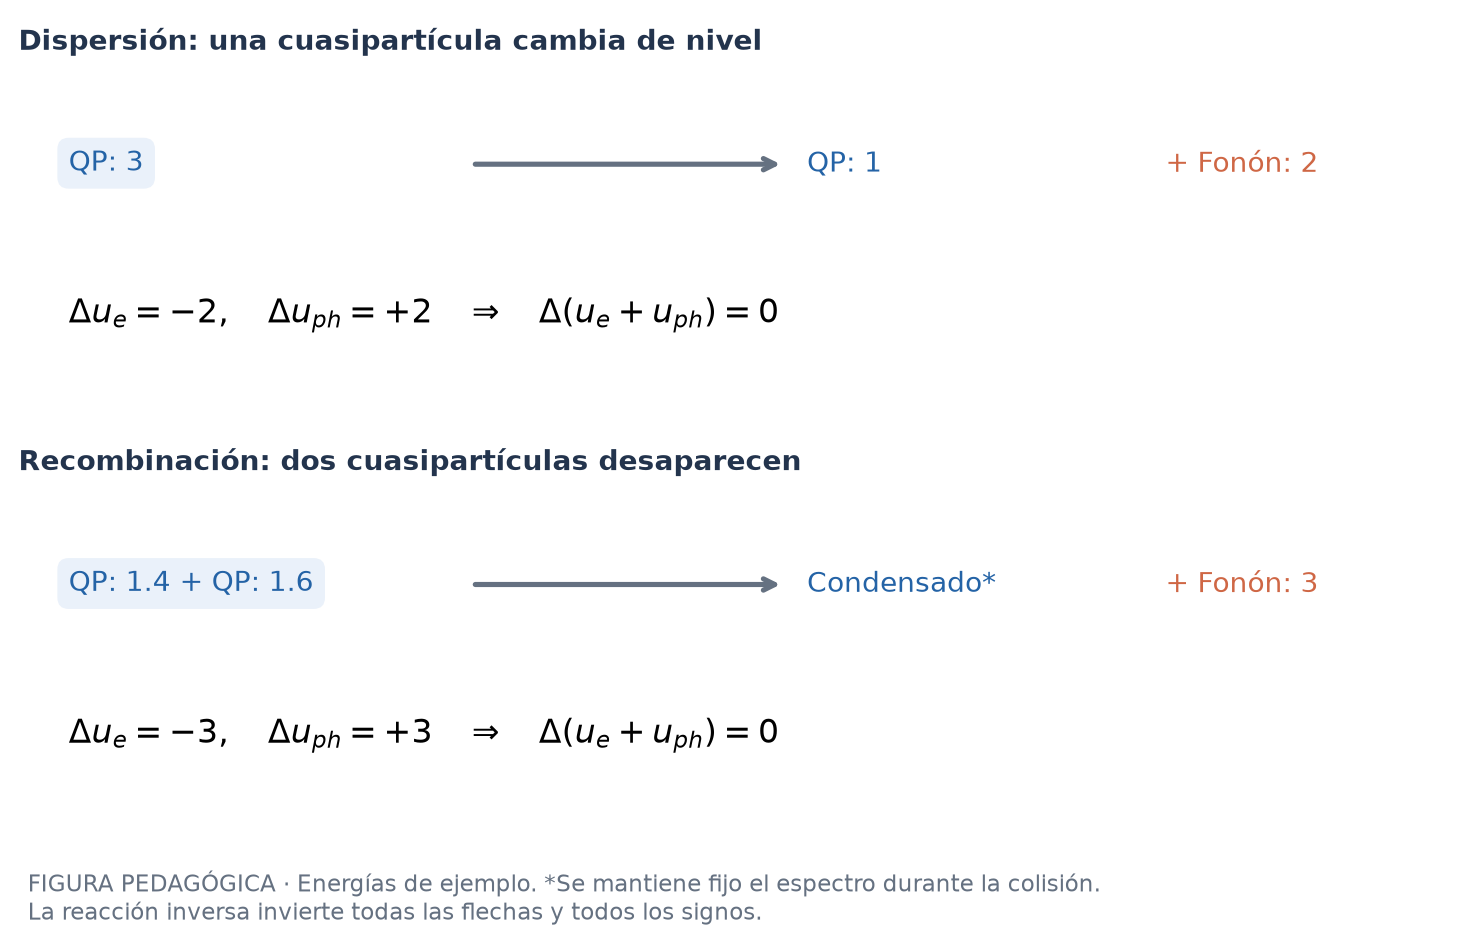
\includegraphics[width=0.96\linewidth,height=\textheight,keepaspectratio,alt={Figura B.1. Recurso pedagógico: cada reacción retira de los electrones exactamente la energía del fonón creado. Las energías son ejemplos arbitrarios; el espectro se mantiene fijo durante la colisión. La recuperación posterior de la amplitud se contabiliza aparte en B.9 y C.}]{../figuras/B_01_reacciones_balance.png}
\caption{Figura B.1. Recurso pedagógico: cada reacción retira de los
electrones exactamente la energía del fonón creado. Las energías son
ejemplos arbitrarios; el espectro se mantiene fijo durante la colisión.
La recuperación posterior de la amplitud se contabiliza aparte en B.9 y
C.}
\end{figure}

\subsection{B.3.1. Factores de
ocupación}\label{b.3.1.-factores-de-ocupaciuxf3n}

Para la emisión neta de un fonón de energía \(\Omega\) por una
cuasipartícula que pasa de \(E+\Omega\) a \(E\),

\[
\mathcal B_S=f(E+\Omega)[1-f(E)](n+1)
-f(E)[1-f(E+\Omega)]n. \tag{B.3}
\]

Para recombinación neta de dos cuasipartículas de energías \(E\) y
\(\Omega-E\),

\[
\mathcal B_R=f(E)f(\Omega-E)(n+1)
-[1-f(E)][1-f(\Omega-E)]n. \tag{B.4}
\]

El signo positivo representa creación neta de fonones; un signo negativo
representa absorción o ruptura de pares.

Cada producto se lee de izquierda a derecha: ocupación inicial,
disponibilidad del estado final y ocupación fonónica. \(1-f\) impide
llegar a un estado electrónico ocupado; \(n+1\) incorpora emisión
espontánea y estimulada. La resta compara el proceso directo con el
inverso. No es necesario asignarles un signo de calentamiento por
separado. Se definen las densidades de reacción, con \(N_0\) por espín,

\[
\begin{gathered}
\mathcal R_S(E,\Omega)=\frac{8\pi N_0}{\hbar}
\alpha^2F(\Omega)\mathcal C_S(E,E+\Omega)\mathcal B_S,\\
0<E<\infty,
\end{gathered} \tag{B.5}
\]

\[
\begin{gathered}
\mathcal R_R(E,\Omega)=\frac{4\pi N_0}{\hbar}
\alpha^2F(\Omega)\mathcal C_R(E,\Omega-E)\mathcal B_R,\\
0<E<\Omega.
\end{gathered} \tag{B.6}
\]

El factor relativo \(1/2\) evita contar dos veces el mismo par al
recorrer \(E\) y \(\Omega-E\). En B.5--B.6, \(\alpha^2F\) tiene la
convención adimensional del eje de energía utilizada en A. Una
implementación que use otra convención debe transformar los prefactores,
no copiar ambas simultáneamente.

\subsection{B.3.2. Ecuación débil para cualquier momento
electrónico}\label{b.3.2.-ecuaciuxf3n-duxe9bil-para-cualquier-momento-electruxf3nico}

Para un peso \(b(E)\), sea

\[
m_b=4N_0\int_0^\infty b(E)\rho(E)f(E)\,dE.
\]

Durante las colisiones, el espectro se mantiene fijo. El cambio debido a
B.5--B.6 es el número neto de reacciones multiplicado por el cambio de
la cantidad observada. En dispersión ese cambio es \(b(E)-b(E+\Omega)\);
en recombinación se pierden ambos pesos. Por tanto,

\[
\begin{aligned}
\left.\dot m_b\right|_{e\text{-ph}}={}&
\int_0^\infty d\Omega\int_0^\infty dE\,
[b(E)-b(E+\Omega)]\mathcal R_S\\
&-\int_0^\infty d\Omega\int_0^\Omega dE\,
[b(E)+b(\Omega-E)]\mathcal R_R.
\end{aligned} \tag{B.7}
\]

Para \(b=1\), la dispersión conserva el número de cuasipartículas y cada
recombinación lo reduce en dos. Para \(b=E\), el corchete de dispersión
vale \(-\Omega\), mientras el de recombinación vale \(\Omega\). Por
tanto,

\[
\left.\dot u_e\right|_{e\text{-ph}}=-P_{e\text{-ph}}, \tag{B.8}
\]

\[
P_{e\text{-ph}}=\int_0^\infty\Omega\left[
\int_0^\infty\mathcal R_S\,dE+
\int_0^\Omega\mathcal R_R\,dE\right]d\Omega. \tag{B.9}
\]

No se decide el signo de la fila fonónica por conveniencia: cada
reacción añade o retira exactamente el fonón que aparece en B.9.

\subsection{B.3.3. Ecuación de
fonones}\label{b.3.3.-ecuaciuxf3n-de-fonones}

Con \(N_iF(\Omega)\) como DOS fonónica por volumen y por energía,

\[
N_iF(\Omega)\dot n(\Omega)=
\int_0^\infty\mathcal R_S\,dE+
\int_0^\Omega\mathcal R_R\,dE
-\frac{N_iF(\Omega)}{\tau_{\rm esc}(\Omega)}[n-n_b]
+S_{\gamma,\rm ph}(\Omega). \tag{B.10}
\]

Su momento energético da

\[
\begin{gathered}
u_{\rm ph}=N_i\int_0^\infty F(\Omega)\Omega n(\Omega)\,d\Omega,\\
\dot u_{\rm ph}=P_{e\text{-ph}}-P_{\rm esc}+S_{\gamma,\rm ph}^{(E)},
\end{gathered} \tag{B.11}
\]

\[
P_{\rm esc}=N_i\int_0^\infty
\frac{F(\Omega)\Omega[n-n_b]}{\tau_{\rm esc}(\Omega)}\,d\Omega. \tag{B.12}
\]

Sin escape ni fuentes, B.8 y B.11 cancelan exactamente el intercambio.
Esta cancelación es independiente de si \(f\) o \(n\) son térmicas. Debe
preservarse al reducir el espectro.

\textbf{Prueba nueva.} Se evaluaron 3000 reacciones de cada tipo con
ocupaciones sintéticas acotadas y pesos positivos. El residuo de
intercambio dividido por la suma de transferencias absolutas es
\(3.96\times10^{-20}\); el máximo residuo de un evento es
\(1.78\times10^{-15}\) en unidades arbitrarias. Es una comprobación
algebraica de signos y contabilidad, no una validación de tasas
materiales.

Un tiempo de escape efectivo único puede mantenerse como primer cierre
de interfaz si se contrasta su efecto sobre los observables de interés.
No se exige un sustrato 3D completo. Tampoco se afirma que una sola
constante reproduzca automáticamente la pérdida de fonones de alta
energía y la relajación tardía. La resolución por rama, ángulo o energía
se promueve cuando el balance o los datos lo requieren {[}A{]}.

\section{B.4. Transporte, evolución del espectro y colisiones
electrón--electrón}\label{b.4.-transporte-evoluciuxf3n-del-espectro-y-colisiones-electruxf3nelectruxf3n}

\textbf{Propósito.} Separar tres cambios que pueden ocurrir
simultáneamente: una ocupación se desplaza en el espacio, una colisión
redistribuye población y el condensado mueve la energía de los estados.
Sólo los dos primeros cambian directamente la población del estado que
se sigue.

\subsection{B.4.1. Difusión electrónica
espectral}\label{b.4.1.-difusiuxf3n-electruxf3nica-espectral}

En el cierre longitudinal de energía de Vodolazov,

\[
\begin{gathered}
\mathcal D_L(E)=N_1^2(E)-R_2^2(E),\\
\boldsymbol\Phi_f(E)=-4N_0D\mathcal D_L(E)\nabla_E f(E).
\end{gathered} \tag{B.13}
\]

La notación \(\nabla_E\) indica una derivada espacial a energía
espectral fija. El flujo de energía es

\[
\mathbf Q_e=\int_0^\infty E\boldsymbol\Phi_f(E)\,dE.
\tag{B.14}
\]

La divergencia del flujo se añade a la ecuación espectral antes de
reducirla. Cuando el peso \(b\) depende de los campos locales, el
momento de transporte es

\[
-\int b\nabla\cdot\boldsymbol\Phi_f\,dE
=-\nabla\cdot\int b\boldsymbol\Phi_f\,dE
+\int(\nabla_Eb)\cdot\boldsymbol\Phi_f\,dE. \tag{B.15}
\]

Ignorar el segundo término para los momentos de fuerza no es una
reducción exacta. B.13 es el sector de energía de la aproximación
adoptada; no sustituye todas las ecuaciones de desequilibrio de carga y
respuesta electromagnética de Keldysh.

\subsection{B.4.2. Derivada temporal a estados
fijos}\label{b.4.2.-derivada-temporal-a-estados-fijos}

Piénsese en pasajeros sobre los peldaños de una escalera mecánica:
cambiar de peldaño y mover la escalera son operaciones diferentes. \(x\)
etiqueta el estado; \(E(x,t)\) es su energía instantánea. En ausencia de
colisiones un estado puede conservar su ocupación aunque cambie la
función dibujada frente al eje \(E\). La regla de la cadena distingue
ambas operaciones.

Con la coordenada \(x\) del documento A,

\[
\begin{gathered}
\left.\dot p\right|_x=
\left.\partial_tf\right|_E+\dot E|_x\,\partial_Ef,\\
\dot E|_x=\frac{R_2}{\rho}\partial_t|\Delta|
-\hbar D\frac{N_2R_2}{\rho}\mathbf q\cdot\dot{\mathbf q}.
\end{gathered} \tag{B.16}
\]

El primer término proporcional a \(\partial_t|\Delta|\) es la estructura
que aparece en la ecuación cinética de Vodolazov. La variación del
espectro no puede omitirse y después compensarse únicamente reajustando
\(C_e\). La misma derivada produce el almacenamiento en amplitud y
superflujo al tomar el momento energético.

Las ecuaciones de ocupación quedan definidas por B.7 para las
reacciones, B.13--B.16 para el transporte y la deriva espectral, y los
operadores adicionales explícitos de electrones y fuentes. Es una
formulación débil equivalente a evolucionar el espectro cuando se
conserva un conjunto completo de pesos. Un número finito de pesos
introduce un cierre nuevo.

\subsection{B.4.3. Un cierre electrónico mínimo que sí conserva
energía}\label{b.4.3.-un-cierre-electruxf3nico-muxednimo-que-suxed-conserva-energuxeda}

La integral electrón--electrón microscópica puede retenerse desde las
fuentes. Como aproximación reducida explícita se propone

\[
\left.\dot p\right|_{ee}
=\frac{f_{\rm FD}(E(x),T_E)-p(x)}{\tau_{ee}(T_E)}. \tag{B.17}
\]

Aquí \(\tau_{ee}\) es constante sobre la energía en una celda y un
instante. \(T_E\) se obtiene por el ajuste energético de B.20. De esta
manera,

\[
4N_0\int E\left.\dot p\right|_{ee}dx=0. \tag{B.18}
\]

Es un cierre de relajación conservativo, no una derivación ab initio de
la interacción Coulomb. Si se introduce \(\tau_{ee}(E)\), la cancelación
B.18 deja de seguir del ajuste energético no ponderado y debe
reformularse el equilibrio objetivo. El cierre tampoco conserva por
imposición un número de cuasipartículas independiente: un modelo con
cuasipotencial químico requeriría declarar y evolucionar esa restricción
adicional.

\section{B.5. Inversión energía--temperatura incluso fuera de
equilibrio}\label{b.5.-inversiuxf3n-energuxedatemperatura-incluso-fuera-de-equilibrio}

\textbf{Propósito.} Disponer de una coordenada energética comparable con
una temperatura, sin afirmar que la distribución ya se haya termalizado.
En una implementación se puede evolucionar \(u_e\) y calcular \(T_E\)
sólo al consultar tablas o mostrar resultados.

\subsection{B.5.1. Definición y prueba de
unicidad}\label{b.5.1.-definiciuxf3n-y-prueba-de-unicidad}

Para el estado electrónico de A,

\[
\begin{gathered}
u_e=U_{\rm vac}(|\Delta|,q)+u_{\rm qp},\\
u_{\rm qp}=4N_0\int_0^\infty E(x)p(x)\,dx.
\end{gathered} \tag{B.19}
\]

Se define \(T_E\) mediante

\[
u_{\rm qp}=4N_0\int_0^\infty
E\rho(E;|\Delta|,q)\frac{dE}{\exp[E/(k_BT_E)]+1}.
\tag{B.20}
\]

A \(|\Delta|,q\) fijos y dentro del catálogo espectral sin autoenergías
explícitamente dependientes de temperatura,

\[
\frac{\partial u_{\rm qp}^{\rm FD}}{\partial T_E}
=\frac{4N_0}{k_BT_E^2}\int_0^\infty
E^2\rho(E)f_{\rm FD}(1-f_{\rm FD})\,dE>0. \tag{B.21}
\]

Luego existe una inversa única dentro del rango energético cubierto.

La deducción usa
\(\partial_T f_{\rm FD}=E f_{\rm FD}(1-f_{\rm FD})/(k_BT^2)\) y
\(\rho\geq0\): todos los sumandos de B.21 son no negativos, con alguno
positivo si existen estados accesibles. Existencia y unicidad se
separan: la monotonía asegura a lo sumo una solución; una energía dentro
de la imagen continua de la función asegura que la solución existe. En
una malla truncada el intervalo permitido es finito y debe comprobarse.
La monotonía no implica buen acondicionamiento a temperatura casi nula,
donde la capacidad puede ser exponencialmente pequeña; eso exige una
representación cuidadosa, no descartar la operación subkelvin.

Si se avanza una energía que incluye \(K_0|\nabla |\Delta||^2\), primero
se resta esa parte y \(U_{\rm vac}\) antes de aplicar B.20. Debe
verificarse que la energía restante pertenece al rango permitido; no se
debe devolver silenciosamente \(T_b\) mediante recorte.

Para fonones, una temperatura equivalente puede definirse por

\[
u_{\rm ph}=N_i\int F(\Omega)\Omega n_B(\Omega,T_{{\rm ph},E})d\Omega.
\tag{B.22}
\]

Su derivada también es positiva. Esa temperatura sirve para describir
energía y presentar resultados. No permite reemplazar una distribución
fonónica no térmica en las tasas de ruptura de pares sin validación.

\begin{figure}
\centering
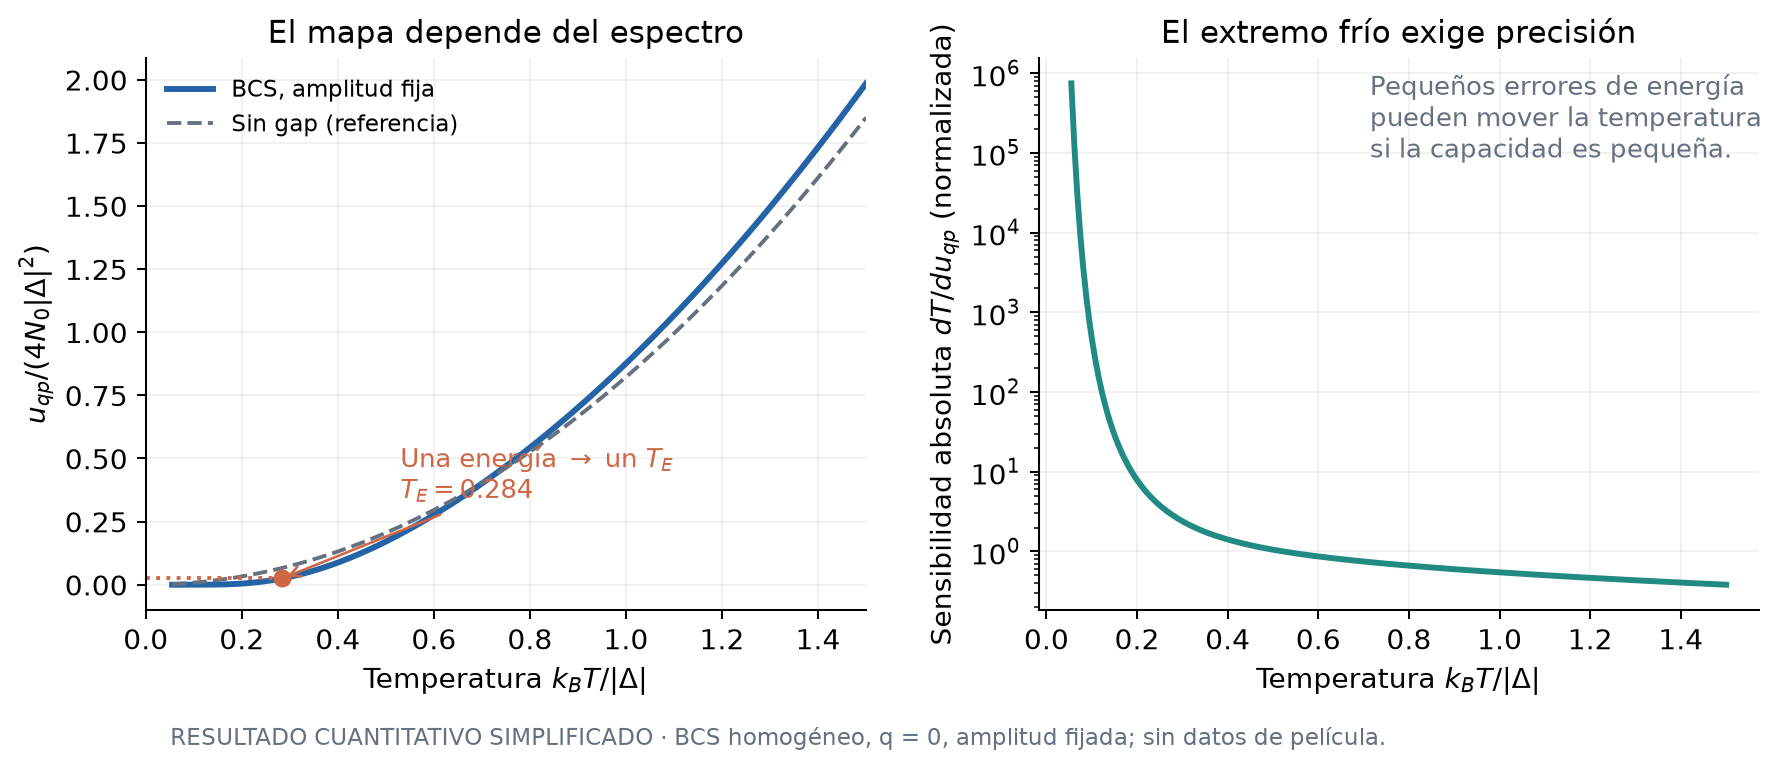
\includegraphics[width=0.98\linewidth,height=\textheight,keepaspectratio,alt={Figura B.2. Resultado cuantitativo de un modelo BCS homogéneo simplificado, con amplitud fija y corriente nula. La curva de energía es invertible; el panel derecho muestra la sensibilidad absoluta de la inversión. La curva sin gap es otro espectro, por eso define otro mapa. No son datos de una película.}]{../figuras/B_02_energia_temperatura.png}
\caption{Figura B.2. Resultado cuantitativo de un modelo BCS homogéneo
simplificado, con amplitud fija y corriente nula. La curva de energía es
invertible; el panel derecho muestra la sensibilidad absoluta de la
inversión. La curva sin gap es otro espectro, por eso define otro mapa.
No son datos de una película.}
\end{figure}

La prueba usa \(x/|\Delta|\in[0,60]\), cuadratura de 1024 puntos y
\(0.055\leq k_BT/|\Delta|\leq1.5\). Al invertir 220 energías se recupera
la temperatura con error absoluto máximo \(2.23\times10^{-16}\) en estas
unidades; refinar de 512 a 1024 puntos cambia la energía menos de
\(1.94\times10^{-13}\) relativo. Es una prueba del mapa a amplitud
impuesta, incluso en regiones donde esa amplitud no sería un equilibrio
autoconsistente.

\subsection{B.5.2. Energía térmica
consistente}\label{b.5.2.-energuxeda-tuxe9rmica-consistente}

Cuando los electrones sí son térmicos,

\[
\begin{gathered}
s_e=-\partial_T f_e^{\rm FD},\\
u_e=f_e^{\rm FD}-T_e\partial_Tf_e^{\rm FD},\\
C_e=-T_e\partial_T^2f_e^{\rm FD}.
\end{gathered} \tag{B.23}
\]

No se diferencia a lo largo de la rama \(|\Delta|_{\rm eq}(T)\) durante
la dinámica. La derivada que convierte energía en temperatura mantiene
el valor instantáneo de \(|\Delta|\) y \(q\). Las otras derivadas se
contabilizan separadamente.

La garantía B.21 corresponde al modelo espectral adiabático definido en
A. Una promoción a autoenergías Eliashberg dependientes de temperatura
exige repetir la prueba con la energía completa. No se hereda
automáticamente la monotonía de una fórmula BCS parcial.

\subsection{B.5.3. Misma energía, otra fuerza sobre el
condensado}\label{b.5.3.-misma-energuxeda-otra-fuerza-sobre-el-condensado}

A \(q=0\), \(E(x)=\sqrt{x^2+|\Delta|^2}\) y la contribución de las
excitaciones a la fuerza es

\[
X_{|\Delta|}^{\rm qp}=4N_0\int_0^\infty\frac{|\Delta|}{E(x)}p(x)\,dx.
\]

El peso de energía es \(E\); el de fuerza es \(|\Delta|/E\). Para un
paquete estrecho, su cociente es \(|\Delta|/E_*^2\): a igual energía
depositada, las excitaciones cercanas al gap pesan más en esta fuerza
que una cola de alta energía. Ésta es la razón matemática por la que el
saldo no basta.

\begin{figure}
\centering
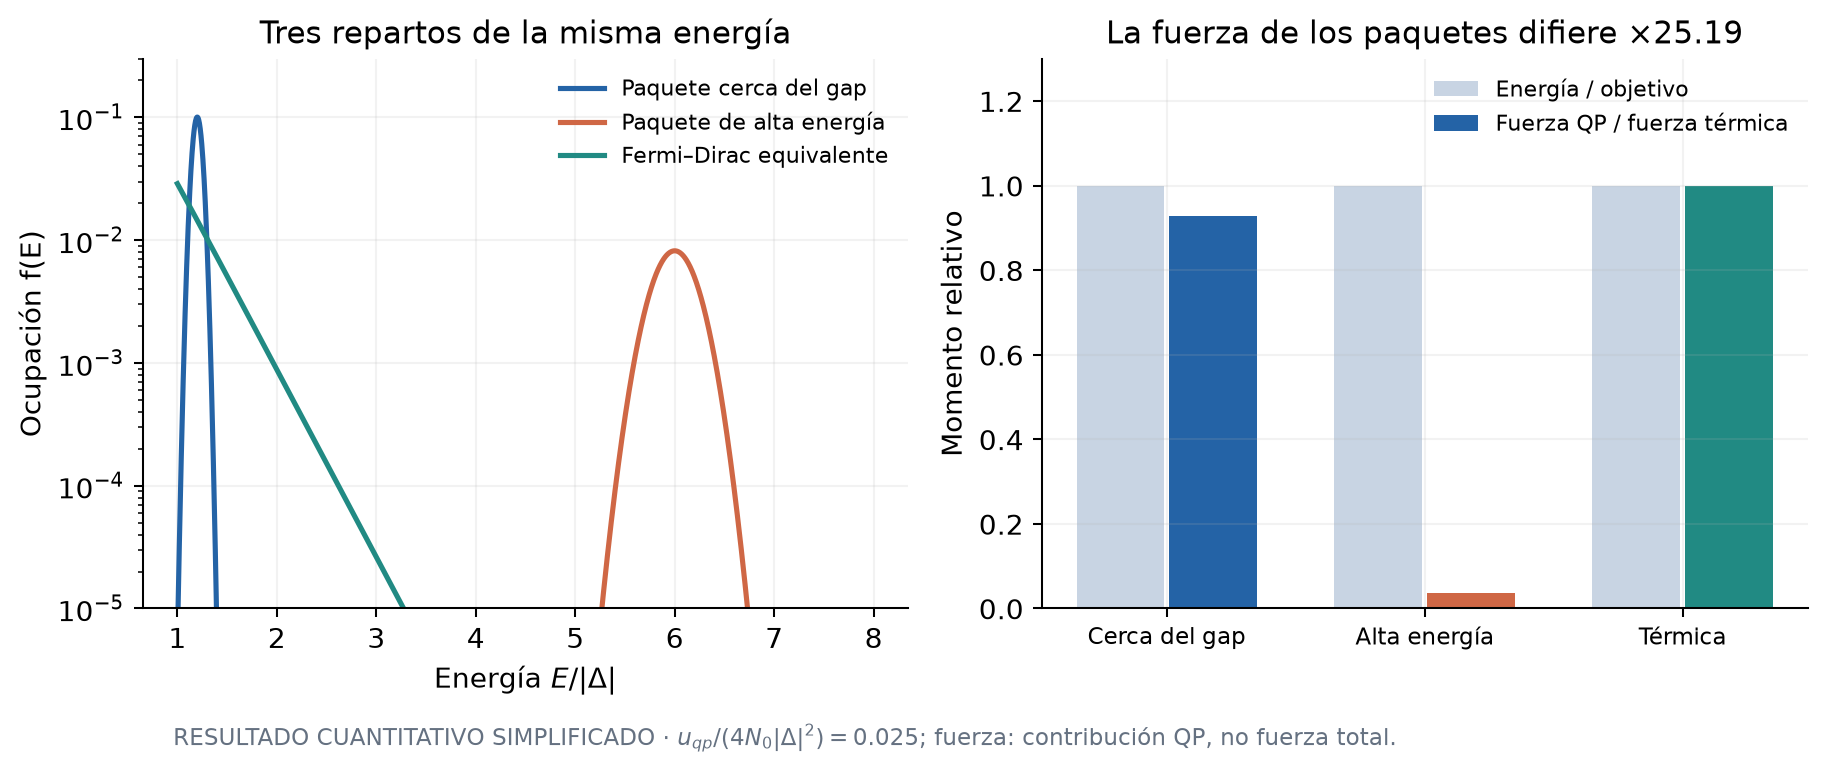
\includegraphics[width=0.98\linewidth,height=\textheight,keepaspectratio,alt={Figura B.3. Resultado cuantitativo simplificado: paquetes gaussianos centrados en 1.2 y 6 veces la amplitud, con anchuras 0.045 y 0.2, y una distribución térmica. Las tres energías coinciden. La barra de fuerza representa sólo la contribución QP; la parte de vacío es común a los tres estados.}]{../figuras/B_03_misma_energia.png}
\caption{Figura B.3. Resultado cuantitativo simplificado: paquetes
gaussianos centrados en 1.2 y 6 veces la amplitud, con anchuras 0.045 y
0.2, y una distribución térmica. Las tres energías coinciden. La barra
de fuerza representa sólo la contribución QP; la parte de vacío es común
a los tres estados.}
\end{figure}

Los tres estados tienen \(u_{\rm qp}/(4N_0|\Delta|^2)=0.025\) y
\(k_BT_E/|\Delta|=0.2844346\). El cociente de fuerzas QP entre los
paquetes es 25.1873. La diferencia es una propiedad de estas poblaciones
sintéticas y de sus pesos BCS; no predice un factor 25 en una latencia
ni reproduce una cascada material.

\section{B.6. Reducción térmica de los integrales sin perder los
espectros
materiales}\label{b.6.-reducciuxf3n-tuxe9rmica-de-los-integrales-sin-perder-los-espectros-materiales}

\textbf{Propósito.} Mostrar qué simplificación se obtiene realmente al
imponer Fermi--Dirac. Se simplifican los factores de ocupación; los
espectros materiales permanecen dentro de los integrales.

Para electrones Fermi--Dirac, las identidades de balance detallado son

\[
\mathcal B_S=[f(E)-f(E+\Omega)]
[n_B(\Omega,T_e)-n(\Omega)], \tag{B.24}
\]

\[
\mathcal B_R=[1-f(E)-f(\Omega-E)]
[n_B(\Omega,T_e)-n(\Omega)]. \tag{B.25}
\]

La segunda se obtiene usando
\((1-f_E)(1-f_{\Omega-E})=e^{\Omega/k_BT_e}f_Ef_{\Omega-E}\).

Para la primera,
\(f(E+\Omega)[1-f(E)]=e^{-\Omega/k_BT_e}f(E)[1-f(E+\Omega)]\). Con
\(n_B=(e^{\Omega/k_BT_e}-1)^{-1}\) se factoriza B.3 y aparece B.24.
Cuando \(n=n_B(T_e)\) ambos balances netos se anulan \textbf{para cada
par de energías}, antes de integrar. Esto es balance detallado; una
potencia integrada cero por cancelación entre canales sería una prueba
más débil. Se definen

\[
J_S(\Omega;T_e,|\Delta|,q)=\int_0^\infty
\mathcal C_S(E,E+\Omega)[f(E)-f(E+\Omega)]\,dE, \tag{B.26}
\]

\[
J_R(\Omega;T_e,|\Delta|,q)=\int_0^\Omega
\mathcal C_R(E,\Omega-E)[1-f(E)-f(\Omega-E)]\,dE. \tag{B.27}
\]

Entonces

\[
\begin{gathered}
\mathcal G_\Omega=\frac{4\pi N_0}{\hbar}\alpha^2F(\Omega)\Omega(2J_S+J_R),\\
P_{e\text{-ph}}=\int_0^\infty\mathcal G_\Omega
[n_B(\Omega,T_e)-n(\Omega)]\,d\Omega.
\end{gathered} \tag{B.28}
\]

La ecuación fonónica se convierte en

\[
\begin{gathered}
\dot n=\gamma_{\rm ph}(\Omega;T_e,|\Delta|,q)
[n_B(\Omega,T_e)-n]-\frac{n-n_b}{\tau_{\rm esc}(\Omega)},\\
\gamma_{\rm ph}=\frac{\mathcal G_\Omega}{N_iF(\Omega)\Omega}.
\end{gathered} \tag{B.29}
\]

Se evalúa el cociente únicamente donde existen modos; fuera de ese
soporte no hay una variable fonónica física que deba dividirse por cero.
En esta versión el catálogo ya no necesita contraer de antemano todo el
espectro a un eje adicional \(T_{\rm ph}\): se pueden conservar tasas
espectrales tabuladas en \((T_e,|\Delta|,q)\).

\subsection{B.6.1. Prueba del límite
normal}\label{b.6.1.-prueba-del-luxedmite-normal}

En el estado normal, \(\mathcal C_S=\mathcal C_R=1\):

\[
\begin{gathered}
J_S=\int_0^\Omega f(E)dE,\\
J_R=\Omega-2\int_0^\Omega f(E)dE.
\end{gathered}
\]

Por tanto,

\[
2J_S+J_R=\Omega. \tag{B.30}
\]

La potencia normal queda

\[
P_{e\text{-ph}}^{n}=\frac{4\pi N_0}{\hbar}
\int_0^\infty\alpha^2F(\Omega)\Omega^2
[n_B(\Omega,T_e)-n(\Omega)]\,d\Omega. \tag{B.31}
\]

Si adicionalmente \(\alpha^2F\propto\Omega^2\) en el intervalo relevante
y los fonones son térmicos, aparece una ley \(T_e^5-T_{\rm ph}^5\). No
debe imponerse esa ley a un espectro completo fuera del intervalo
acústico correspondiente.

\begin{figure}
\centering
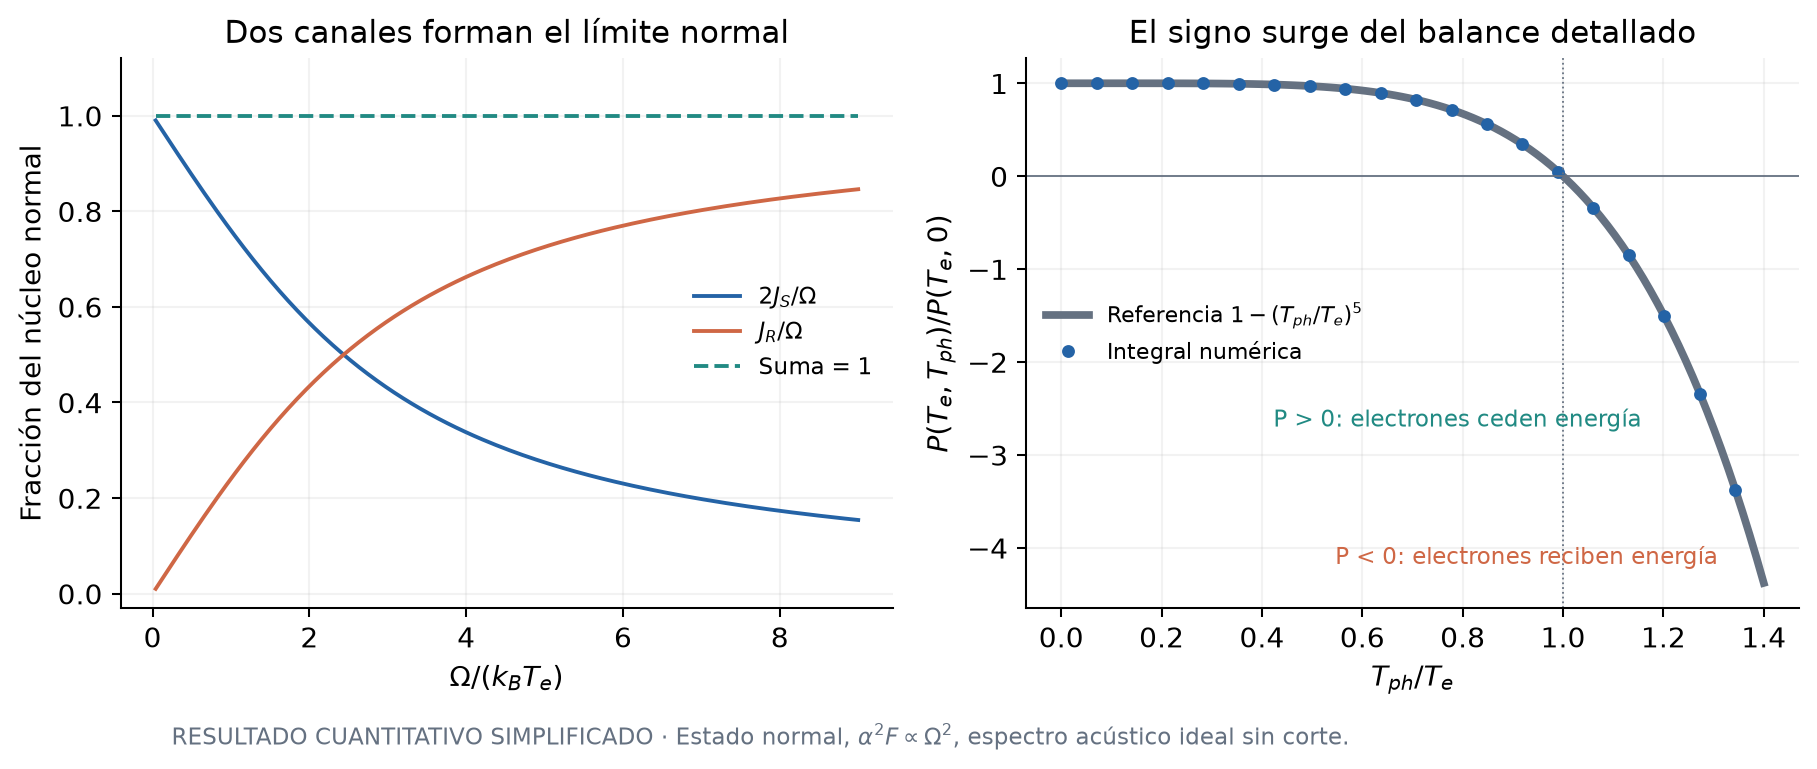
\includegraphics[width=0.98\linewidth,height=\textheight,keepaspectratio,alt={Figura B.4. Resultado cuantitativo simplificado del límite normal. Izquierda: los dos canales suman exactamente el núcleo normal. Derecha: para un espectro acústico ideal, la integral cambia de signo cuando los fonones superan la temperatura electrónica. La ley de quinta potencia es una referencia de este límite, no un ajuste impuesto al material.}]{../figuras/B_04_limite_normal.png}
\caption{Figura B.4. Resultado cuantitativo simplificado del límite
normal. Izquierda: los dos canales suman exactamente el núcleo normal.
Derecha: para un espectro acústico ideal, la integral cambia de signo
cuando los fonones superan la temperatura electrónica. La ley de quinta
potencia es una referencia de este límite, no un ajuste impuesto al
material.}
\end{figure}

Integrando por separado B.26 y B.27, el error relativo máximo de
\(2J_S+J_R=\Omega\) es \(7.02\times10^{-14}\). Para el espectro acústico
ideal, el error absoluto máximo de \(P/P(T_e,0)=1-(T_{\rm ph}/T_e)^5\)
es \(4.71\times10^{-14}\). Los factores originales y reducidos
B.24--B.25 coinciden a \(2.50\times10^{-15}\) absoluto en los casos de
prueba.

\subsection{B.6.2. Conductividad térmica del mismo
espectro}\label{b.6.2.-conductividad-tuxe9rmica-del-mismo-espectro}

Al insertar \(\nabla f=(\partial f/\partial T_e)\nabla T_e\) en B.14,

\[
\kappa_s(T_e,|\Delta|,q)=\frac{4N_0D}{k_BT_e^2}
\int_0^\infty E^2\mathcal D_L(E)
 f_{\rm FD}(1-f_{\rm FD})\,dE. \tag{B.32}
\]

Con \(\mathcal D_L=1\), se recupera
\(\kappa_n=(\pi^2k_B^2/3e^2)\sigma_nT_e\). Esta prueba verifica
simultáneamente unidades, espín y normalización. La expresión nueva
retiene la dependencia de depairing que no estaba presente en la
conductividad BCS \(\kappa_s(T_e,|\Delta|)\) de producción.

\section{B.7. Cómo reducir sin borrar la física que se desea
mejorar}\label{b.7.-cuxf3mo-reducir-sin-borrar-la-fuxedsica-que-se-desea-mejorar}

\textbf{Propósito.} Reducir coste sólo después de verificar las
magnitudes que afectan al detector. Dos distribuciones pueden verse
similares en energía y diferir en una fuerza o una tasa; la figura B.3
es un contraejemplo mínimo.

\subsection{B.7.1. Criterio de paso a electrones
térmicos}\label{b.7.1.-criterio-de-paso-a-electrones-tuxe9rmicos}

Se compara el estado espectral con \(f_{\rm FD}(T_E)\) manteniendo
\((|\Delta|,q)\) idénticos. Deben ser pequeños los errores de
\(X_{|\Delta|}\), \(j_s\) y \(P_{e\text{-ph}}\); además se controla el
flujo de energía. La igualdad de \(u_e\) es exacta por construcción y no
sirve como única prueba del cierre.

Se proponen tolerancias iniciales del 3--5\% en magnitudes dinámicamente
relevantes, con denominadores regularizados mediante escalas físicas
cuando la cantidad se anula. Son criterios de aceptación del proyecto,
no constantes universales. Se exige permanencia durante un intervalo y
se comprueba que el cambio de representación no modifica la energía, la
fuerza ni la corriente de forma discontinua. Si los criterios fallan, se
retiene el espectro; no se fuerza la termalización por alcanzar cierto
número de picosegundos.

\subsection{B.7.2. Cierre de máxima entropía: derivación y
límite}\label{b.7.2.-cierre-de-muxe1xima-entropuxeda-derivaciuxf3n-y-luxedmite}

Para intentar una reducción finita se pueden conservar momentos de
energía y de fuerzas:

\[
\begin{gathered}
b_1(x)=E(x),\\
b_2(x)=\partial_{|\Delta|}E(x),\\
b_3(x)=\partial_qE(x),\\
m_\alpha=4N_0\int b_\alpha p\,dx.
\end{gathered} \tag{B.33}
\]

Se maximiza la entropía de A.20 fijando los \(m_\alpha\). Absorbiendo
\(k_B\) en los multiplicadores, la variación local da

\[
\ln\frac{1-p(x)}{p(x)}-\sum_\alpha\lambda_\alpha b_\alpha(x)=0.
\]

Despejar \(p\) conduce a

\[
p_{\boldsymbol\lambda}(x)=
\frac1{1+\exp[\sum_\alpha\lambda_\alpha b_\alpha(x)]}. \tag{B.34}
\]

El Jacobiano negativo del mapa de multiplicadores a momentos es

\[
\begin{gathered}
H_{\alpha\beta}=4N_0\int b_\alpha b_\beta p(1-p)\,dx,\\
\mathbf v^TH\mathbf v=4N_0\int(\mathbf v\cdot\mathbf b)^2p(1-p)dx\geq0.
\end{gathered} \tag{B.35}
\]

La independencia de los pesos sobre los estados poblados da positividad
estricta y unicidad local. En \(q=0\) el tercer peso puede anularse; se
elimina esa restricción degenerada. No se invierte una matriz singular
añadiendo una supuesta nueva física.

Los pesos se mueven cuando cambia el condensado:

\[
\begin{aligned}
\dot m_\alpha={}&4N_0\int b_\alpha\dot p\,dx\\
&+4N_0\int(\partial_{|\Delta|}b_\alpha\partial_t|\Delta|+
\partial_{\mathbf q}b_\alpha\cdot\dot{\mathbf q})p\,dx.
\end{aligned}\tag{B.36}
\]

Se combinan B.7, B.15 y B.36 para obtener el sistema reducido. Esto
expone todos los términos omitidos por una proyección ingenua sobre
energía solamente. La técnica de máxima entropía está respaldada por la
teoría de cierres cinéticos {[}L{]}; la selección concreta de pesos B.33
y su aplicación al SNSPD son propuestas de este desarrollo.

\textbf{Estado de validación en 0.2.} La figura B.3 verifica que energía
sola no fija la fuerza. No se ha ejecutado en esta revisión un ajuste de
máxima entropía ni la comparación de sus integrales electrón--fonón con
un espectro material. Los errores del 24\% y 67\% citados en 0.1 no se
mantienen como resultados revalidados, porque sus archivos de cálculo no
acompañan a los documentos recibidos. La positividad de B.35 garantiza
propiedades del ajuste; no garantiza que las tasas omitidas sean
precisas.

\subsection{B.7.3. Fonones por bandas}\label{b.7.3.-fonones-por-bandas}

Para una banda \(B_b\) se conserva su energía

\[
\begin{gathered}
U_b=N_i\int_{B_b}F(\Omega)\Omega n(\Omega)d\Omega,\\
\dot U_b=P_b-P_{{\rm esc},b}+S_{\gamma,b}.
\end{gathered} \tag{B.37}
\]

\(P_b\) debe ser exactamente la contribución retirada de los electrones.
La reconstrucción intrabanda ---por ejemplo, máxima entropía
restringida--- debe declararse y comprobarse aumentando el número de
bandas. Las bandas se eligen atendiendo a umbrales y estructura de
\(\alpha^2F\), no a una temperatura Debye que borre el espectro
original.

\section{B.8. Condición inicial tras la
absorción}\label{b.8.-condiciuxf3n-inicial-tras-la-absorciuxf3n}

\textbf{Propósito.} Declarar qué energía y qué distribución entrega la
parte no resuelta de la cascada al intervalo que sí se modela. Conocer
la energía del fotón normaliza la condición inicial, pero no determina
su forma espectral ni su extensión espacial.

El fotón ya está absorbido. No se calcula aquí su probabilidad de
absorción ni la eficiencia del instrumento. Una densidad inicial
\(u_\gamma(\mathbf r)\) satisface

\[
\int_{\mathcal V}u_\gamma(\mathbf r)dV=E_\gamma. \tag{B.38}
\]

Se consideran dos condiciones tempranas documentadas: una excitación
electrón--hueco de alta energía dentro del rango en que el operador
cinético utilizado sea válido, o una burbuja fonónica como
representación posterior a una parte de la cascada no resuelta. Ninguna
se confunde con una distribución Bose caliente por tener una energía
conocida.

Una forma espectral motivada por la ponderación de acoplamiento es
\(\delta n\propto\alpha^2(\Omega)=\alpha^2F(\Omega)/F(\Omega)\). Su
normalización energética es

\[
\delta n(\Omega,\mathbf r)=
\frac{u_\gamma(\mathbf r)\,\alpha^2(\Omega)}
{N_i\int_0^\infty\Omega\alpha^2F(\Omega)d\Omega}.
\tag{B.39}
\]

B.39 define una condición de transferencia entre descripciones, no un
resultado único sobre la absorción óptica ni una predicción universal de
la distribución tras cada fotón. El perfil espacial inicial y el tiempo
de transferencia deben contrastarse con soluciones cinéticas tempranas
{[}S, A{]}. El condensado puede iniciarse continuo y evolucionar
mediante su fuerza no térmica; no se impone un salto instantáneo a su
mínimo de equilibrio.

Si se resuelve el escape durante esa etapa, no se multiplica
adicionalmente la energía por una fracción retenida que contabilice la
misma pérdida. Si una etapa anterior queda fuera del modelo, se declara
qué energía entrega al intervalo resuelto y qué incertidumbre temporal
deja. La publicación debe distinguir el tiempo relativo de esa condición
inicial del instante óptico absoluto.

La gaussiana truncada en un borde no debe renormalizarse sin discutir el
mecanismo de confinamiento o escape: energía total absorbida, energía
retenida en el volumen y forma espacial son datos diferentes. Esto no
exige resolver óptica; exige no convertir una conveniencia geométrica en
una ley de la cascada.

\section{B.9. Energía del condensado y fuentes de
calentamiento}\label{b.9.-energuxeda-del-condensado-y-fuentes-de-calentamiento}

\textbf{Propósito.} Evitar que recuperar amplitud cree o destruya
energía en el balance total. La energía del estado de fondo y la de las
excitaciones son partes distintas de la misma contabilidad electrónica.

El balance de una celda no se cierra sumando a la ecuación antigua dos
derivadas de almacenamiento y conservando sin cambios todas las fuentes.
La potencia reversible de superflujo, la disipación del parámetro de
orden y el trabajo eléctrico deben contarse una vez. C deriva la
identidad completa.

Para electrones térmicos, la forma resultante es

\[
\begin{aligned}
C_e\dot T_e={}&\nabla\cdot(\kappa_s\nabla T_e)
+\sigma_nE^2+Q_\Delta\\
&-P_{e\text{-ph}}+S_{\gamma,e}^{(E)}\\
&+T_e f_{T|\Delta|}\partial_t|\Delta|+T_e\partial_T\partial_{\mathbf q}f\cdot\dot{\mathbf q}.
\end{aligned}
\tag{B.40}
\]

\(f=f_e^{\rm FD}\) y \(Q_\Delta\geq0\) es la disipación del condensado.

\(S_{\gamma,e}^{(E)}\) representa una fuente electrónica resuelta; vale
cero si la absorción ya quedó incorporada como condición inicial. Los
subíndices de \(f\) indican derivadas parciales:
\(f_{T|\Delta|}=\partial_T\partial_{|\Delta|}f\). Es una ecuación
invertible y consistente con el funcional, no un uso ad hoc de
\(j_s\cdot E\) como calentamiento siempre positivo.

En la fase espectral, la energía \(P_{\rm heat}=\sigma_nE^2+Q_\Delta\)
necesita una distribución entre estados. Una opción de cierre explícita,
conservativa en energía, es

\[
\left.\dot p\right|_{\rm heat}
=\frac{P_{\rm heat}\,E(x)p(1-p)}
{4N_0\int_0^\infty E^2p(1-p)dx}. \tag{B.41}
\]

Su momento energético vale \(P_{\rm heat}\) y en el límite térmico sigue
la dirección de calentamiento de Fermi--Dirac. \textbf{B.41 no es la
integral microscópica exacta de calentamiento eléctrico fuera de
equilibrio.} Es un cierre térmicamente orientado para la energía
disipada; su efecto durante el intervalo no térmico debe compararse con
un tratamiento cinético más completo. Cuando ese calentamiento temprano
es despreciable frente a la cascada, el error asociado puede acotarse.
Si no lo es, B.41 no debe ocultarse dentro de una supuesta derivación ab
initio.

\subsection{B.9.1. Celda aislada como prueba de
almacenamiento}\label{b.9.1.-celda-aislada-como-prueba-de-almacenamiento}

Para una celda homogénea sin corriente, fuentes, escape ni intercambio
fonónico, C da \(\partial_t|\Delta|=-\mathcal M X_{|\Delta|}\) y
\(Q_\Delta=\mathcal M X_{|\Delta|}^2\). Aquí
\(\mathcal M=1/\Gamma_{|\Delta|}>0\) es la movilidad, inversa de la
fricción de C. De \(u_e=f-Tf_T\) se obtiene, a \(q=0\),

\[
\dot u_e=(X_{|\Delta|}-T f_{T|\Delta|})\partial_t|\Delta|
+C_e\dot T.
\tag{B.42}
\]

Al sustituir B.40 se cancelan los términos mixtos y queda
\(\dot u_e=X_{|\Delta|}\partial_t|\Delta|+Q_\Delta=0\). Esta cancelación
explica el calentamiento durante la recuperación sin convertir todo el
cambio de amplitud en una fuente térmica adicional.

\textbf{Prueba nueva, instantánea.} Se evalúa una celda BCS a
\(|\Delta|/\Delta_0=0.4\), \(k_BT/\Delta_0=0.08\) y movilidad positiva
unitaria en unidades de tiempo arbitrarias. Se obtiene fuerza negativa,
recuperación de amplitud, \(Q_\Delta>0\) y \(\dot T>0\); el residuo de
B.42 resulta cero a la precisión registrada. La prueba evalúa derivadas
locales; no integra una trayectoria ni predice una temperatura final
material. C añade una trayectoria de un modelo de celda simplificado
para visualizar esta transferencia.

Las cifras finales de amplitud y temperatura de la celda citada en 0.1
no se presentan como revalidadas. La ecuación B.42 de esta versión
sustituye aquella referencia numérica por una identidad verificable con
los archivos entregados.

\section{B.10. Criterios de aceptación antes del transitorio
2D}\label{b.10.-criterios-de-aceptaciuxf3n-antes-del-transitorio-2d}

Las comprobaciones ligeras realizadas en 0.2 son condiciones necesarias
para avanzar. Sus residuos miden las pruebas concretas, no el error
físico de un detector.

{\def\LTcaptype{none} % do not increment counter
\begin{longtable}[]{@{}
  >{\raggedright\arraybackslash}p{(\linewidth - 4\tabcolsep) * \real{0.3333}}
  >{\raggedright\arraybackslash}p{(\linewidth - 4\tabcolsep) * \real{0.3333}}
  >{\raggedright\arraybackslash}p{(\linewidth - 4\tabcolsep) * \real{0.3333}}@{}}
\toprule\noalign{}
\begin{minipage}[b]{\linewidth}\raggedright
Verificación nueva
\end{minipage} & \begin{minipage}[b]{\linewidth}\raggedright
Resultado
\end{minipage} & \begin{minipage}[b]{\linewidth}\raggedright
Alcance
\end{minipage} \\
\midrule\noalign{}
\endhead
\bottomrule\noalign{}
\endlastfoot
Intercambio de 6000 reacciones sintéticas & Residuo relativo
\(3.96\times10^{-20}\) & Contabilidad de eventos a espectro fijo \\
Balance detallado de B.3 y B.4 & Residuo absoluto máximo
\(2.23\times10^{-15}\) & Distribuciones térmicas con temperatura
común \\
Energía BCS e inversión & Error de temperatura
\(\leq2.23\times10^{-16}\) & 220 temperaturas, amplitud fija, \(q=0\) \\
Paquetes de igual energía & Fuerza QP: cociente 25.1873 & Poblaciones
sintéticas declaradas \\
Límite normal B.30 & Error relativo \(7.02\times10^{-14}\) & DOS normal
constante \\
Ley de quinta potencia & Error normalizado \(4.71\times10^{-14}\) &
Espectro acústico ideal \\
Celda aislada, B.42 & Cancelación a precisión registrada & Identidad
instantánea, sin transitorio \\
\end{longtable}
}

Falta validar el núcleo material completo, su no negatividad, la
discretización que conserva energía al desplazar el espectro, el límite
normal de B.32 dentro de la implementación futura y el cierre de pocos
momentos contra una referencia espectral. La comparación de cascadas
debe medir energía electrónica y fonónica, fuerza \(X_{|\Delta|}\),
corriente, escape acumulado y persistencia del error de reducción.

No se ejecutaron los datos DFT de producción ni un transitorio espacial
en estas comprobaciones. Los archivos verificables de esta revisión son
\nolinkurl{sandbox/model_v0_2/checks_b.py},
\nolinkurl{verificaciones/B_verificaciones.json}, seis tablas CSV con
prefijo \nolinkurl{B_}, y cuatro figuras PNG/PDF. Los originales 0.1 se
conservan como antecedentes; las cifras nuevas tienen su propio registro
de procedencia.

\section{Referencias y procedencia}\label{referencias-y-procedencia}

{[}M{]} J. A. Díaz Monge, \nolinkurl{memoria_02.pdf}, 2026, anexo B,
pp.~impresas 113--120; anexo A.5 para la aproximación de coherencia.
Estado térmico de producción: \(P_\Delta\) y \(P_q\) omitidos y
deposición inicial en \(T_{\rm ph}\).

{[}V{]} D. Y. Vodolazov, Physical Review Applied \textbf{7}, 034014
(2017). DOI: 10.1103/PhysRevApplied.7.034014; arXiv:1611.06060.
Ecuaciones cinéticas espectrales y su reducción.

{[}S{]} A. Simon et al., Physical Review B \textbf{112}, 174512 (2025).
DOI: 10.1103/3m2k-mzr6; arXiv:2501.13791. Espectros materiales y
cinética no equilibrada.

{[}A{]} J. P. Allmaras, \nolinkurl{Allmaras_thesis.pdf}, capítulos 2 y 3,
especialmente pp.~impresas 49--53, 91--94 y 101--114. Comparaciones
entre cinética, modelos térmicos y burbuja fonónica modificada.

{[}L{]} C. D. Levermore, \emph{Moment closure hierarchies for kinetic
theories}, Journal of Statistical Physics \textbf{83}, 1021--1065
(1996). Marco de cierres por momentos y entropía. La base B.33 y los
criterios para este SNSPD no se atribuyen a ese artículo.

{[}R{]} Inspección histórica de 0.1: \nolinkurl{JoaquinDiazM/pysnspd},
revisión \nolinkurl{f3c26b95ff4e4a93504371e78b46ad3a20e06273}; sectores
\nolinkurl{thermal/evolution.py}, \nolinkurl{kinetic/phase_space.py},
\nolinkurl{kinetic/power_table.py} y \nolinkurl{excitation/photon.py}. Las
verificaciones nuevas son independientes del solver y se identifican en
{[}Q{]}; D registra la revisión local de contexto.

{[}Q{]} Verificaciones nuevas de 0.2:
\nolinkurl{sandbox/model_v0_2/checks_b.py},
\nolinkurl{verificaciones/B_verificaciones.json} y CSV/figuras con prefijo
\nolinkurl{B_}. Los scripts mencionados en 0.1 no se presuponen
disponibles ni reejecutados. Los documentos A y C fijan,
respectivamente, el funcional y el balance de disipación utilizados
aquí.

\end{document}
